\epigraph{\textit{It doesn't matter how beautiful your theory is, it doesn't matter how smart you are. If it doesn't agree with the experiment, it's wrong.}}{-- \textup{Richard P. Feynman }}

In the following chapter, a description of the theoretical concepts needed for a proper understanding of this document is done. Ranging from \textit{knowledge graphs} to \textit{data-flow paradigms}, we are providing a firm foundation for the experiment to be conducted.

\section{Knowledge graphs}
\label{section:knowledgeGraph}

A knowledge graph uses a graph-structured data model to represent knowledge of some real-world domain. Where each node represents an entity -- a \textit{thing} from the actual world -- and the edges are the relationships between them. This type of graph is often assembled from a wide variety of sources, and as a result, can be highly diverse in terms of structure and granularity~\cite{DBLP:journals/corr/abs-2003-02320}. To address this issue, representations of \textit{schema}, \textit{identity} and \textit{context} are needed. While the former defines the high-level structure of the graph, \textit{identity} relates nodes that conform to the same real-world entity; finally, \textit{context} provides the environment for specific knowledge to be understood. Let me write a more formal definition of a knowledge graph:

\begin{definition}[Knowledge Graph]
    A knowledge graph is a graph-structured data model that captures knowledge in a specific domain, having nodes that represent entities and edges that represent relationships between their entities~\cite{https://doi.org/10.48550/arxiv.2110.11709}.
\end{definition}

Note that the definition above is as general as it gets. In this manner, a knowledge graph can be represented using different technologies. In the following sections, we will focus on the most representative examples of knowledge graphs: \textit{RDF graphs} and \textit{property graphs}. We will also discuss the \textit{Wikibase} data model, as it is the one used in the experiment to be conducted.

\subsection{RDF (Resource Description Framework) graphs}
\label{section:RDF}

Let me first introduce \textit{Resource Description Framework} (RDF) as it is the most simple and widely used technology for representing a knowledge graph model. RDF is a data interchange W3C standard for the web. It has been used as a method for the description and exchange of graph data\footnote{\url{https://en.wikipedia.org/wiki/Resource_Description_Framework}}, providing a variety of syntax notations and formats, with \texttt{Turtle} being the most adopted one. One of the main features of RDF is that it allows the combination of different data sources, even if the schemas differ from one another. What's more, it supports the evolution of schemas without requiring the data consumers to adapt to those changes.

RDF is a directed graph composed of triple statements; called \textit{semantic triples}, in the way of \textit{subject-predicate-object}. Where each element is identified by a URI. The \textit{subject} denotes the resource you want to make statements about, the \textit{predicate} denotes attributes of the resource and models relationships among the \textit{subject} and the \textit{object}, and the \textit{object} is the value of the attribute. As an example, we can represent that \textit{the genre of The Hunger Games is dystopian fiction} in RDF as the triple: a \textbf{subject} denoting \textit{The Hunger Games}, a \textbf{predicate} denoting \textit{is of genre}, and an \textbf{object} denoting \textit{dystopian fiction}. This representation can be seen in Figure \ref{fig:RDF}.

\begin{figure}[ht]
    \centering
    \includestandalone[width=0.8\textwidth]{diagrams/6-4_RDF}
    \caption{Directed knowledge graph generated out of a triple \textit{subject-predicate-object}}
    \label{fig:RDF}
\end{figure}

We have mentioned that the most common syntax notation for RDF is Turtle; however, one of the simplest is N-Triples. Each line of a \texttt{.nt} document is a single triple \textit{subject-predicate-object}, followed by a full stop, meaning the termination of the statement. All that together form a directed knowledge graph. Let's see an example of an RDF graph represented using N-Triples notation.

\begin{example}[RDF knowledge graph using N-Triples notation]
    \href{https://www.wikidata.org/entity/Q7251}{Alan Turing (Q7251)} \href{https://www.wikidata.org/entity/P19}{was born (P19)} in \href{https://www.wikidata.org/entity/Q20895942}{Warrington Lodge (Q20895942)} and \href{https://www.wikidataWShEx.org/entity/P108}{was employed (P108)} by the \href{https://www.wikidata.org/entity/Q220798}{Government of the United Kingdom (Q220798)} where he \href{https://www.wikidata.org/entity/P61}{discovered (P61)} the Enigma-deciphering machine \href{https://www.wikidata.org/entity/Q480476}{bombe (Q480476)}.
\end{example}

\begin{dumps}
    \inputminted{turtle}{code/listings/6-3_serialization.nt}
\end{dumps}

\subsection{Property graphs}

A property graph is a type of graph model where vertices and edges, namely nodes and relationships, are annotated with labels and properties. In this manner, property graphs excel at depicting connections between data and exposing data dependencies. When compared to other \textit{datastores}, such as relational databases, property graphs focus on how the recorded things relate, although descriptions of those items might be supplied via properties and attributes. In this sense, provided a real-world domain, expressing the relationships among data is just as crucial as the data itself.

With that in mind, it can be argued that there's no need for a new type of \textit{datastore} as relational databases are capable of storing those relationships through constraints. However expensive operations such as \texttt{JOIN} are required to navigate across those links. It turns out that relational databases handle relationships between data in a not-so-sophisticated manner. To tackle this issue, graph databases were created. In this model, relationships are stored natively alongside the nodes in a flexible format. Several commercial graph databases like Neo4j\footnote{\url{https://neo4j.com/}}, JanusGraph\footnote{\url{https://janusgraph.org/}} or Sparksee\footnote{\url{https://www.sparsity-technologies.com/\#sparksee}} were developed.

\begin{figure}[ht]
    \centering
    \includestandalone[width=0.8\textwidth]{diagrams/6-1_propertyGraph}
    \caption{Example of a property graph}
    \label{fig:propertyGraph}
\end{figure}

Note that figure \ref{fig:propertyGraph} is a simplified version of a property graph. This is because what we have tried here is to extend the example in figure \ref{fig:RDF} transforming the RDF graph into a property one.

\label{section:wikibase_graphs}
\subsection{Wikibase graphs}

Wikidata started back in 2012 as a support to Wikipedia. Rapidly becoming one of the biggest human knowledge bases, with remarkable organizations donating their data to it; as an example, Google migrated \textit{Freebase} -- its previous knowledge graph -- to Wikidata in 2017~\cite{10.1145/2872427.2874809}. As of October 9, 2022, Wikidata currently contains roughly 100 million items\footnote{\url{https://www.wikidata.org/wiki/Wikidata:Statistics}}. Internally, Wikidata's content is stored in a SQL database (MariaDB); however, this system is not ideal for querying or data analysis. With that in mind, and pursuing the integration of Wikibase within the semantic web ecosystem, the Wikimedia Foundation adopted BlazeGraph: an open-source triple store and graph database\footnote{\url{https://en.wikipedia.org/wiki/Blazegraph}}. This way, two data models coexist in Wikibase: a document-centric model based on MediaWiki, and an RDF-based one that can be used to perform SPARQL queries through the Query Service~\cite{https://doi.org/10.48550/arxiv.2110.11709}.

\begin{figure}[ht]
    \centering
    \includestandalone[width=0.5\textwidth]{diagrams/6-2_architectureWikibase}
    \caption[Simplified architecture of Wikibase]{Simplified architecture of Wikibase~\cite{https://doi.org/10.48550/arxiv.2110.11709}}
    \label{fig:architecture:wikibase}
\end{figure}

Informally speaking, the Wikibase data model is composed of \textit{entities} and \textit{statements} (about those entities). This way, an entity can be either an \textit{item} or a \textit{property}. Items are used to represent all the \textit{things} from human knowledge. Usually denoted by a \texttt{Q} followed by a sequence of digits; as an example, \href{https://www.wikidata.org/wiki/Q7251}{Q7251} represents Alan Turing in Wikidata. On the other hand, properties model a relationship between an item and a value, and are represented by a \texttt{P} followed by a sequence of numbers; as an example, \href{https://www.wikidata.org/wiki/Property:P31}{P31} is the property \textit{instance of} in Wikidata.

For values to be associated with properties, they must belong to some specific data type\footnote{\url{https://www.wikidata.org/wiki/Help:Data_type}}. Supported data types include URLs, time, quantities, and mathematical expressions; to name a few. Notice how more complex data types are also supported; those include \textit{properties} and \textit{items}, this way, relationships among entities are allowed.

Lastly, a statement is a piece of data about an item and is recorded on the page of the item itself. Putting it all together, the way Wikibase manages information is as follows: through a statement, we add information to a certain item using some property and its value. This can be seen in figure \ref{fig:wikibaseStatement}.

\begin{figure}[ht]
    \centering
    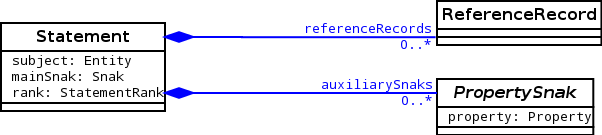
\includegraphics[width=.8\linewidth]{figures/diagrams/6-11_statement.png}
    \caption[Formal definition of a statement in Wikibase]{Formal definition of a statement in Wikibase\footnotemark}
    \label{fig:wikibaseStatement}
\end{figure}
\footnotetext{\url{https://www.mediawiki.org/wiki/Wikibase/DataModel\#Statements}}

The different components that appear in figure \ref{fig:wikibaseStatement} are as follows:

\begin{itemize}
    \itemsep0.25em
    \item \textbf{Subject}: the item to which the statement refers.
    \item \textbf{mainSnak}: the main \textit{property-value} pair for a certain entity.
    \item \textbf{Rank}: to tell if a certain \texttt{Statement} is \texttt{deprecated} or not.
    \item \textbf{referenceRecords}: a list of references that support the statement.
    \item \textbf{qualifierSnaks}: a list of qualifiers that modify the meaning of the statement.
\end{itemize}

This may seem to be a complex data model, but it is not. It is quite simple indeed. To illustrate this, we will use an example.

\begin{example}[Adding information to an entity in Wikidata\footnote{\url{https://www.wikidata.org/wiki/Help:Statements}}]
    \label{example:wikibaseGraph}
    To include information about the genre of \textit{The Hunger Games} in Wikidata, we would need to add a statement to the item itself: \href{https://www.wikidata.org/wiki/Q11679}{The Hunger Games (Q11679)}, using the property \href{https://www.wikidata.org/wiki/Property:P136}{genre (P136)}, we can then add the value \href{https://www.wikidata.org/wiki/Q15062348}{dystopian fiction (Q15062348)}. Notice how we are linking two entities (\textit{items}) of the Wikidata.
\end{example}

\begin{table}[ht]
    \centering
    \documentclass{standalone}
\usepackage[table,xcdraw]{xcolor}
\usepackage{varioref,multicol}
\usepackage{hyperref}  
\begin{document}
\begin{tabular}{|c|l|l|l|}
    \hline
    \rowcolor[HTML]{EFEFEF}
    \textbf{Language} & \multicolumn{1}{c|}{\cellcolor[HTML]{EFEFEF}\textbf{Item}}                              & \multicolumn{1}{c|}{\cellcolor[HTML]{EFEFEF}\textbf{Property}}                            & \multicolumn{1}{c|}{\cellcolor[HTML]{EFEFEF}\textbf{Value}}                             \\ \hline
    \textit{English}  & \multicolumn{1}{l|}{\href{https://www.wikidata.org/wiki/Q11678}{The Hunger Games}}      & \multicolumn{1}{l|}{\href{https://www.wikidata.org/wiki/Property:P136}{genre}}            & \multicolumn{1}{l|}{\href{https://www.wikidata.org/wiki/Q15062348}{dystopian fiction}}  \\ \hline
    \textit{Spanish}  & \multicolumn{1}{l|}{\href{https://www.wikidata.org/wiki/Q11678}{Los juegos del hambre}} & \multicolumn{1}{l|}{\href{https://www.wikidata.org/wiki/Property:P136}{género}}           & \multicolumn{1}{l|}{\href{https://www.wikidata.org/wiki/Q15062348}{ficción distópica}}  \\ \hline
    \textit{French}   & \multicolumn{1}{l|}{ \href{https://www.wikidata.org/wiki/Q11678}{Hunger Games}}         & \multicolumn{1}{l|}{\href{https://www.wikidata.org/wiki/Property:P136}{genre artistique}} & \multicolumn{1}{l|}{\href{https://www.wikidata.org/wiki/Q15062348}{fiction dystopique}} \\ \hline
    \textit{Wikidata} & \multicolumn{1}{c|}{\href{https://www.wikidata.org/wiki/Q11678}{Q11678}}                & \multicolumn{1}{c|}{\href{https://www.wikidata.org/wiki/Property:P136}{P136}}             & \multicolumn{1}{c|}{\href{https://www.wikidata.org/wiki/Q15062348}{Q15062348}}          \\ \cline{2-4}
\end{tabular}
\end{document}
    \caption[Including information about the genre of \textit{The Hunger Games}]{Including information about the genre of \textit{The Hunger Games}\footnotemark}
    \label{tab:language}
\end{table}
\footnotetext{\url{https://www.wikidata.org/wiki/Q11678}}

\subsubsection{Opaque URIs}
\label{section:opaqueURIs}

Recall that the main purpose of Wikidata is to store data about things that are described by pages in Wikipedia (in any language)\footnote{\url{https://www.mediawiki.org/wiki/Wikibase/DataModel}}. This means, \textit{things} should be represented in such a way that they don't depend on the natural language used; that is, language independence is required. In Wikidata, this is achieved through a linked data pattern called \textit{opaque URIs}. In general, a URI is defined as a unique sequence of characters that identifies the resources of the system\footnote{\url{https://en.wikipedia.org/wiki/Uniform_Resource_Identifier}}. Designing good URIs is the first step in linked data development.

The characters that appear in a URI tend to be related to the concept they represent, improving human readability. As an example, \texttt{https://example.com/España} could -- potentially -- be an identifier for the Spanish country. However, for those non-Spanish speakers, that identifier is meaningless. What's more, the use of non-ASCII characters may lead to problems in an internationalized system. Opposed to \textit{descriptive URIs}, \textit{opaque} ones are not intended to represent terms in a natural language~\cite{LabraGayo2015MultilingualLD}. An example of that is \url{https://www.wikidata.org/wiki/Q11679}, where item \texttt{Q11679} represents \textit{The Hunger Games} in Wikidata. However -- in some situations -- it is helpful for users to interact with human-readable names. In Wikidata, this is solved through \textit{labels}, which are language-dependent. Following the previous example, the label tagged to the entity \texttt{Q11679} is the actual title of the book: \textit{The Hunger Games}. Translations for several languages can also be provided. Notice table~\ref{tab:language} for an example of possible \textit{labels} for some \textit{opaque URIs}.

What we have seen so far is an overview of the Wikibase \textit{data model}; including: \textit{statements}, \textit{properties}, \textit{values} and the appropriate mechanism for identifying them (in a multilingual approach). The next step is to formally define what a Wikibase graph is.

\begin{definition}[Wikibase graphs]
    Given a mutually disjoint set of items $\mathcal{Q}$, a mutually disjoint set of properties $\mathcal{P}$, and a mutually disjoint set of values $\mathcal{V}$, a Wikibase graph is a quadruple $(\mathcal{Q}, \mathcal{P}, \mathcal{V}, \rho)$. Where $\rho \subseteq \mathcal{Q} \times \mathcal{P} \times \mathcal{V}$ is a set of statements.
\end{definition}

For a better understanding of this formal definition, let me explain it step-by-step. Any \textit{item} in $\mathcal{Q}$ can have information added to it using $\mathcal{Q}$ \textit{entities}, $\mathcal{P}$ \textit{properties}, or $\mathcal{V}$ \textit{data values}. Meaning that we can add a statement about a particular entity in $\mathcal{Q}$ using the aforementioned set of values. For us to provide extra information to a certain relationship, we may include it in the fourth entry of the quadruples in the $\rho$ set, see example \ref{example:knowledgeGraph} for more details. As an example, to establish the \href{https://www.wikidata.org/wiki/Property:P585}{point in time} at which \href{https://www.wikidata.org/wiki/Q937} {Albert Einstein} received the \href{https://www.wikidata.org/wiki/Q38104}{Nobel Prize in Physics}, we may annotate the \href{https://www.wikidata.org/wiki/Property:P166}{award received} property with the value 1921\footnote{\url{https://www.nobelprize.org/prizes/physics/1921/summary/}}. Those are called \textit{qualifiers}. For further clarification, let us model the Wikibase graph of a certain scenario.

\vspace*{-0.5em}

\begin{example}[Wikibase Knowledge Graph]
    \label{example:knowledgeGraph}
    We are willing to qualify that Alan Turing (23 June 1912 -- 7 June 1954) was employed by the government of the United Kingdom in the course of WWII. During that time he invented the computer for deciphering Enigma-machine-encrypted secret messages\footnote{\url{https://en.wikipedia.org/wiki/Bombe}}. Additional information about relevant places where he lived is also annotated.
\end{example}

\vspace*{-1.25em}

% Tikz File 'fig_03_wikibaseGraph.tex'
\documentclass{standalone}
\usepackage{tikz}
\usepackage{../mystyle}
\newcommand{\myfont}[1]{\ensuremath{\mathcal{#1}}}

\newcommand{\triple}[3]{\ensuremath{\langle #1,#2,#3 \rangle}}
\newcommand{\quadruple}[4]{\ensuremath{\langle #1,#2,#3,#4\rangle}}

\newcommand{\ItemSet}{\myfont{Q}}
\newcommand{\PropSet}{\myfont{P}}
\newcommand{\EntitySet}{\myfont{E}}
\newcommand{\ValueSet}{\myfont{V}}
\newcommand{\DataValueSet}{\myfont{D}}
\newcommand{\StmtSet}{\rho}
\newcommand{\FinSet}[1]{\ensuremath{FinSet(#1)}}

\newcommand{\hrefc}[3][blue]{\href{#2}{\color{#1}{#3}}}%

\newcommand{\elemento}[2]{\ensuremath{\hrefc[violet]{http://www.wikidata.org/entity/#2}{#1}}}
\newcommand{\propiedad}[2]{\ensuremath{\hrefc[blue]{http://www.wikidata.org/entity/#2}{#1}}}
\newcommand{\alanTuring}{\elemento{alanTuring}{Q7251}}
\newcommand{\wilmslow}{\elemento{wilmslow}{Q2011497}}
\newcommand{\town}{\elemento{town}{Q3957}}
\newcommand{\government}{\elemento{government}{Q220798}}
\newcommand{\warringtonLodge}{\elemento{warringtonLodge}{Q20895942}}
\newcommand{\bombe}{\elemento{bombe}{Q480476}}
\newcommand{\unitedKingdom}{\elemento{unitedKingdom}{Q145}}
\newcommand{\computer}{\elemento{computer}{Q11742076}}
\newcommand{\dateOfBirth}{\propiedad{dateOfBirth}{P569}}
\newcommand{\placeOfBirth}{\propiedad{placeOfBirth}{P19}}
\newcommand{\country}{\propiedad{country}{P27}}
\newcommand{\employer}{\propiedad{employer}{P108}}
\newcommand{\discoverer}{\propiedad{discoverer}{P61}}
\newcommand{\dateOfDeath}{\propiedad{dateOfDeath}{P570}}
\newcommand{\placeOfDeath}{\propiedad{placeOfDeath}{P20}}
\newcommand{\timeStart}{\propiedad{timeStart}{P580}}
\newcommand{\timeEnd}{\propiedad{timeEnd}{P582}}
\newcommand{\manufacturer}{\propiedad{manufacturer}{P176}}
\newcommand{\Human}{\elemento{Human}{Q5}}
\newcommand{\instanceOf}{\propiedad{instanceOf}{P31}}

\setlength{\tabcolsep}{1mm}
\renewcommand{\arraystretch}{1.5}
\usetikzlibrary{positioning,arrows}
\begin{document}
\begin{tikzpicture}[
        vertex/.style={
                rectangle,
                rounded corners,
                draw=black!60,
                fill=black!5,
                minimum width=15mm,
                minimum height=7.5mm,
                text centered,
                font=\footnotesize
            },
        predicate/.style = {font=\footnotesize\ttfamily},
        >= stealth',
        shorten >= 0.5pt
    ]
    \node[vertex,align=center] (alanTuring) at (-2, 0) {\alanTuring\\{\tiny \dateOfBirth  \hspace{1mm} \textit{23 June 1912}}\\{\tiny \dateOfDeath  \hspace{1mm} \textit{7 June 1954}}};
    \node[vertex] (human) at (-2, -2) {\Human};
    \node[vertex] (birth) at (2.75, 2.25) {\warringtonLodge};
    \node[vertex] (death) at (1, 4) {\wilmslow};
    \node[vertex] (employer) at (4, 0) {\government};
    \node[vertex] (country) at (7.25, 2.25) {\unitedKingdom};
    \node[vertex] (bombe) at (4, -2) {\bombe};
    \node[vertex] (machine) at (1, -3.25) {\computer};
    \node[vertex] (town) at (6, 4) {\town};

    \path[->] (alanTuring.north) edge[bend left] node[predicate,sloped,above] {\placeOfDeath} (death.west);
    \path[->] (alanTuring.north) edge[bend left] node[predicate,sloped,above] {\placeOfBirth} (birth.west);
    \path[->] (alanTuring.south) edge node[predicate,left] {\instanceOf} (human.north);
    \path[->] (alanTuring.east) edge node[label={[align=left,font=\tiny]above:\employer\\- \timeStart \hspace{1mm} \textit{1938}\\- \timeEnd \hspace{1mm} \textit{1945}}] {} (employer.west);
    \path[->] (birth.east) edge node[predicate,sloped,above] {\country} (country.west);
    \path[->] (bombe.south) edge[bend left] node[predicate,sloped,below] {\instanceOf} (machine);
    \path[->] (bombe.north) edge node[predicate,left] {\manufacturer} (employer.south);
    \path[->] (bombe) edge[bend left] node[predicate,sloped,above] {\discoverer} (alanTuring);
    \path[->] (bombe.east) edge[bend right] node[predicate,sloped,above] {\country} (country);
    \path[->] (death.east) edge node[predicate,above] {\instanceOf} (town.west);
    \path[->] (death) edge node[predicate,sloped,above] {\country} (country);
\end{tikzpicture}
\end{document}

\begin{figure}[H]
    \centering
    \includestandalone[width=0.9\textwidth]{diagrams/6-3_wikibaseGraph}
    \caption[Formal description and visualization of Turing's Wikibase graph]{Formal description and visualization of Turing's Wikibase graph}
\end{figure}

\subsubsection{Wikibase data serialization}
\label{section:wikibase:serialization}

The Wikibase data model supports two export formats, namely, JSON and RDF. Being the former the one employed by the JSON dumps and the latter follows semantic web and linked data principles. A fragment of both formats is shown below. According to the following example:

\begin{example}[Seralization of a node using JSON and RDF]
    \href{https://www.wikidata.org/wiki/Q7251}{Alan Turing (Q7251)} was \href{https://www.wikidata.org/wiki/Property:P108}{employed (P108)} by the \href{https://www.wikidata.org/wiki/Q220798}{Government Communications Headquarters (Q220798)} of the United Kingdom, during the World War II (1938-1945).
\end{example}

\paragraph{Wikibase JSON serialization}

The JSON serialization follows the Wikibase data model~\cite{https://doi.org/10.48550/arxiv.2110.11709}. Consisting of a sequence of items where each element is a JSON object capturing all the information about the item itself, represented in a single line. What's remarkable about this mechanism is that it records all the neighboring (see definition \ref{definition:neighborhood}) entities of every single node, making algorithms that validate whole graphs able to process them in a single pass. More on this will be discussed in paragraph \ref{section:pregel}.

\begin{dumps}
    \inputminted{json}{code/listings/6-1_serialization.json}
\end{dumps}

As a human-readable format is useful for data communication, the REST API architecture is growing in popularity. Consequently, JSON format has swiftly gained acceptance since it's perfectly suited for speedy data sharing. Nevertheless, since so much boilerplate code is produced, in the Big data world, JSON-based apps may suffer from performance issues. Take note of how information is kept in a JSON file: as key-value pairs for each item. As a result, a JSON document that stores objects of the same type will have the same number of columns as the number of items in the document. Hence, one of the major flaws of this serialization format is the lack of memory optimization, which means JSON is not even remotely compact. Putting it all together, JSON outperforms binary formats in situations where a person must go through the file; yet, for our purposes, columnar-based formats work just better than row-oriented ones.

\paragraph[Wikibase RDF serialization]{Wikibase RDF serialization\footnotemark}
\footnotetext{\url{https://www.wikidata.org/wiki/Special:EntityData/Q7251.ttl}}

The RDF serialization of Wikidata\footnote{\url{https://www.mediawiki.org/wiki/Wikibase/Indexing/RDF_Dump_Format}} is mainly used by the Wikidata's Query Service described in Figure \ref{fig:architecture:wikibase}. The main goal of this format is to provide support for semantic web technologies. See section \ref{section:RDF} for further details.

\begin{dumps}
    \inputminted{turtle}{code/listings/6-2_serialization.rdf}
\end{dumps}

\section{Knowledge Graph validation}

As a brief introduction to this section, let's first describe what validation -- in the context of Knowledge graphs -- is. Wikibase is a collection of data that anyone can edit. This can lead to some concerns regarding the integrity of what is posted on Wikibase, as there is no single point of truth for any given piece of information. According to this, for some piece of data to be considered valid, its description needs to be both syntactically correct and adhere to some type-definition. As we have seen in section \ref{section:wikibase:serialization}, the different serialization formats supported by Wikidata include RDF as one of those. Putting it all together, we require a mechanism for ensuring the \textit{validity} of the RDF documents stored in Wikibase.

\subsection{ShEx (Shape Expressions)}

Shape Expressions (ShEx) were designed as a high-level, domain-specific language for describing RDF graph structures~\cite{https://doi.org/10.48550/arxiv.2110.11709}. The syntax of ShEx is inspired by Turtle and SPARQL, while the semantics are inspired by RelaxNG and XML Schema. In this manner, Shape Expressions specify the requirements that RDF data graphs must fulfill to be regarded as conformant, including which elements should appear in a given graph and with what cardinalities and data types\footnote{\url{https://shexspec.github.io/primer/}}.

\begin{figure}[ht]
    \centering
    
\includegraphics[width=.125\linewidth]{img/6-1_shex.png}
    \caption{ShEx data validation language}
\end{figure}

A ShEx schema is used to validate an RDF graph in the ShEx model, which then identifies the portions of the graph that fail to conform to the schema. What's more, schemas allow systems to establish contracts for sharing information; this way, through a common schema, several systems may agree that a certain element should appear in some entity. This pattern behaves similarly to interfaces in the object-oriented paradigm. Lastly, the shapes can be specified using any RDF serialization language, such as JSON-LD or Turtle, or a human-friendly concise syntax called ShExC.

\label{code:shex}
\begin{code}[ShExC syntax example declaring that nodes of the shape Person must fulfill a schema]
    \inputminted{shexc}{code/listings/6-4_shex.shex}
\end{code}

Following the previous example, another possibility is to visualize ShEx schemas using UML-like class diagrams, we are using a tool called \href{https://rdfshape.weso.es/shexInfo}{RDF Shape} for creating the schema. This way, the representation seen in Figure \ref{fig:RDFshape} arises.

\begin{figure}[ht]
    \centering
    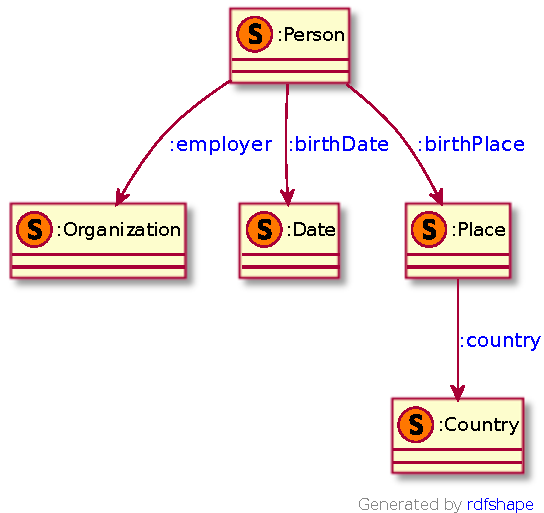
\includegraphics[width=0.4\textwidth]{diagrams/6-5_ShEx.pdf}
    \caption{ShEx schema visualization as UML-like diagrams}
    \label{fig:RDFshape}
\end{figure}

The FAIR (\fb{Findable}, \fb{Accessible}, \fb{Interoperable} and \fb{Reusable}) Guiding principles for data management state that as data's amount, complexity, and rate of creation rise, humans will increasingly need computational assistance to manage it\footnote{\url{https://www.go-fair.org/fair-principles/}}. This is where Wikidata Schemas, or WShEx, could help us address that issue. Wikidata's dumps can be examined in this manner to see if they adhere to a particular schema, obtaining a subset of valid entities as a result. Thus, the community can exchange and reuse data from Wikidata by using schemas, which also serve to improve the quality and usefulness of the data.

ShEx was chosen by Wikibase in 2019 to be the language for describing entity schemas\footnote{\url{https://www.wikidata.org/wiki/Wikidata:Database_reports/EntitySchema_directory}}. As ShEx cannot be used for JSON validation, instead of the Wikibase data model itself, Shape Expressions describe the RDF serialization of Wikibase entities. This implies that the ShEx-based approach is far from the Wikibase data model itself. This issue will be fixed through the solution described in section \ref{section:WShEx}. Observe how the opaque URIs we discussed in section \ref{section:opaqueURIs} are used as the identifiers for specifying Wikidata items.

\begin{code}[ShExC syntax example declaring that nodes of the shape Person must fulfill a schema]
    \inputminted{shex}{code/listings/6-5_wikibase.shex}
\end{code}

\subsubsection{WShEx}
\label{section:WShEx}

As a solution to the problem described before, an extension of ShEx for describing the Wikibase data model was designed. WShEx is a language inspired by ShEx that provides support for the Wikibase data model and can be used to describe and validate Wikibase entities~\cite{https://doi.org/10.48550/arxiv.2208.02697}. What's more, the main motivation for developing this language was to create subsets of Wikidata using a human-readable language.

\begin{code}[ShExC syntax example declaring that nodes of the shape Person must fulfill a schema]
    \inputminted{shex}{code/listings/6-6_wshex.shex}
\end{code}

Figure \ref{fig:WShEx} represents the relationship between ShEx, WShEx and the Wikibase data model. This way, by validating the Wikibase data model through WShEx, we are not only validating the dumps but the system itself.

\begin{figure}[ht]
    \centering
    \includestandalone[width=0.6\textwidth]{diagrams/6-6_WShEx}
    \caption[Relationships between ShEx, WShEx and the Wikibase data model]{Relationships between ShEx, WShEx and the Wikibase data model~\cite{https://doi.org/10.48550/arxiv.2110.11709}}
    \label{fig:WShEx}
\end{figure}

\section{Knowledge Graph Subsets}

Wikidata keeps getting bigger and better. A vast volume of data, like that found in Wikidata, has several benefits but also some drawbacks, including performance. One approach that also provides a snapshot of the contents of Wikidata at a specific point in time is to replicate Wikidata on one's infrastructure~\cite{10.37044/osf.io/wu9et}. However, replicating Wikidata in its entirety is not necessary; instead, subsets might be used to focus on, say, a specific domain. As a substitute for reducing the volume and range of data given by Wikidata, those subsets have become more popular. While maintaining compatibility with the entire Wikidata as the model is retained, handling fewer data enables more complex searches and operations over it.

\begin{definition}[Wikibase subset~\cite{https://doi.org/10.48550/arxiv.2110.11709}]
    Given a Wikibase graph $\Graph=\langle\ItemSet,\PropSet,\DataValueSet,\StmtSet\rangle$, a Wikibase sub-graph is defined as  $\Graph'=\langle\ItemSet',\PropSet',\DataValueSet',\StmtSet'\rangle$ such that: $\ItemSet'\subseteq\ItemSet$, $\PropSet'\subseteq\PropSet$, $\DataValueSet'\subseteq\DataValueSet$ and $\StmtSet'\subseteq\StmtSet$.
\end{definition}

\begin{example}[Example of wikibase subgraph]
    Given the Wikibase graph $\Graph=\langle\ItemSet,\PropSet,\DataValueSet,\StmtSet\rangle$ from example \ref{example:wikibaseGraph}, $\Graph'=\langle\ItemSet',\PropSet',\DataValueSet',\StmtSet'\rangle$ is a Wikibase subgraph of $\Graph$.
\end{example}

\begin{table}[ht]
    \centering
    \documentclass{standalone}
\usepackage{longtable}
% creating some commands for reuse later on :D
\newcommand{\myfont}[1]{\ensuremath{\mathcal{#1}}}

\newcommand{\VertSet}{\myfont{V}}
\newcommand{\NodeSet}{\myfont{N}}
\newcommand{\EdgeSet}{\myfont{E}}
\newcommand{\LabelSet}{\myfont{L}}
\newcommand{\PLabelSet}{\myfont{T}}
\newcommand{\MsgSet}{\myfont{M}}
\newcommand{\None}{\myfont{None}}

\newcommand{\triple}[3]{\ensuremath{\langle #1,#2,#3 \rangle}}
\newcommand{\quadruple}[4]{\ensuremath{\langle #1,#2,#3,#4\rangle}}
\newcommand{\ItemSet}{\myfont{Q}}
\newcommand{\PropSet}{\myfont{P}}
\newcommand{\EntitySet}{\myfont{E}}
\newcommand{\ValueSet}{\myfont{V}}
\newcommand{\DataValueSet}{\myfont{D}}
\newcommand{\StmtSet}{\rho}
\newcommand{\FinSet}[1]{\ensuremath{FinSet(#1)}}
\newcommand{\Graph}{\myfont{G}}

\newcommand{\hrefc}[3][blue]{\href{#2}{\color{#1}{#3}}}%
\newcommand{\elemento}[2]{\ensuremath{\hrefc[violet]{http://www.wikidata.org/entity/#2}{#1}}}
\newcommand{\propiedad}[2]{\ensuremath{\hrefc[blue]{http://www.wikidata.org/entity/#2}{#1}}}
\newcommand{\alanTuring}{\elemento{alanTuring}{Q7251}}
\newcommand{\wilmslow}{\elemento{wilmslow}{Q2011497}}
\newcommand{\town}{\elemento{town}{Q3957}}
\newcommand{\government}{\elemento{government}{Q220798}}
\newcommand{\warringtonLodge}{\elemento{warringtonLodge}{Q20895942}}
\newcommand{\bombe}{\elemento{bombe}{Q480476}}
\newcommand{\unitedKingdom}{\elemento{unitedKingdom}{Q145}}
\newcommand{\computer}{\elemento{computer}{Q11742076}}
\newcommand{\dateOfBirth}{\propiedad{dateOfBirth}{P569}}
\newcommand{\placeOfBirth}{\propiedad{placeOfBirth}{P19}}
\newcommand{\country}{\propiedad{country}{P27}}
\newcommand{\employer}{\propiedad{employer}{P108}}
\newcommand{\discoverer}{\propiedad{discoverer}{P61}}
\newcommand{\dateOfDeath}{\propiedad{dateOfDeath}{P570}}
\newcommand{\placeOfDeath}{\propiedad{placeOfDeath}{P20}}
\newcommand{\timeStart}{\propiedad{timeStart}{P580}}
\newcommand{\timeEnd}{\propiedad{timeEnd}{P582}}
\newcommand{\manufacturer}{\propiedad{manufacturer}{P176}}
\newcommand{\Human}{\elemento{Human}{Q5}}
\newcommand{\instanceOf}{\propiedad{instanceOf}{P31}}

\newcommand{\fb}[1]{\dofb#1}
\newcommand{\dofb}[1]{\textbf{#1}\nobreak\hspace{0pt}}

\newcommand{\mi}[1]{\ensuremath{\mathit{#1}}}

\newcommand{\emptyGraph}{\ensuremath{\emptyset}}
\newcommand{\EmptyGraph}{\ensuremath{\emptyset}}
\newcommand{\addTriple}{\ensuremath{\rtimes}}
\newcommand{\unionGraphs}{\ensuremath{\cup}}
\newcommand\neighs[2]{\ensuremath{neighs(#1,#2)}}
\newcommand\nodes[1]{\ensuremath{nodes(#1)}}
\newcommand{\node}{\mi{n}}
\newcommand{\lbl}{\mi{l}}
\newcommand{\g}{\mi{g}}
\newcommand{\vertex}{\mi{v}}
\newcommand{\msg}{\mi{msg}}
\newcommand{\msgs}{\mi{msgs}}
\newcommand{\labels}{\mi{labels}}
\newcommand{\TripleConstraint}{\mi{TripleConstraint}}
\newcommand{\ShapeReference}{\mi{ShapeReference}}
\newcommand{\ShapeAnd}{\mi{ShapeAnd}}
\newcommand{\ShapeOr}{\mi{ShapeOr}}
\newcommand{\Cardinality}{\mi{Cardinality}}

% Algorithmic definitions
\SetKwProg{Def}{def}{$\,$:}{}
\SetKwProg{Defn}{def}{~$=$}{}
\SetKw{defn}{def}
\newcommand{\DefInline}[2]{\defn #1 = #2}
\SetKwProg{DefnCustom}{\defn}{}{}
\SetKw{Let}{let}
\SetKwInput{KwIn}{Input}
\SetKwFor{ForEach}{foreach}{}{}
\SetKw{Or}{or}
\SetKw{And}{and}
\SetKwIF{If}{ElseIf}{Else}{if}{then}{else if}{else}{endif}
\SetKw{Match}{match}
\SetKw{MyIf}{if}
\SetKw{MyThen}{then}
\SetKw{MyElse}{else}
\SetKw{Case}{case}
\SetKwBlock{Let}{let}{in}
\SetKw{In}{in}
\SetKw{MapTo}{\ensuremath{\;\;\Rightarrow\;\;}}
\SetKwBlock{Block}{}{}
\newcommand{\assign}{\ensuremath{~\mathtt{:=}~}}
\newcommand{\algocomment}[1]{\text{//$\,$#1}}

\newcommand{\blockskip}{\smallskip}
\newcommand{\done}{\ensuremath{\mathit{done}}}

% [algorithm spacing:]
\def\algorithmsize{small}
\def\algorithmheadersize{\algorithmsize}
\renewcommand\AlCapFnt{\normalfont\bfseries\small}
\setlength{\textfloatsep}{1.0ex}
\setlength{\floatsep}{1.0ex}

% Statuses
\newcommand{\Ok}{\ensuremath{Ok}}
\newcommand{\Failed}{\ensuremath{Failed}}
\newcommand{\WaitingFor}[3]{\ensuremath{WaitingFor}(#1,#2,#3)}
\newcommand{\Pending}{\ensuremath{Pending}}
\newcommand{\PendingLs}{\ensuremath{Pending}(ls)}
\newcommand{\Undefined}{\ensuremath{Undefined}}

\newcommand{\Validate}{\ensuremath{Validate}}
\newcommand{\Checked}[2]{\ensuremath{Checked(#1,#2)}}
\newcommand{\WaitFor}[1]{\ensuremath{WaitFor(#1)}}
\newcommand{\status}[2]{\ensuremath{#1(#2)}}
\newcommand{\msgSent}[3]{\ensuremath{#1,#2\rightsquigarrow{}#3}}
\newcommand{\checkLocal}[2]{\ensuremath{checkLocal(#1,#2)}}
\newcommand{\checkLocalOpen}[2]{\ensuremath{checkLocalOpen(#1,#2)}}

\newcommand{\neighbors}[3]{\ensuremath{neighbors}(#1,#2,#3)}
\newcommand{\fracEmpty}[2]{\genfrac{}{}{0pt}{0}{#1}{#2}}
\newcommand{\vProg}{vProg}
\newcommand{\tripleConstraints}[1]{tripleConstraints(#1)}
\newcommand{\rbe}[1]{\ensuremath{rbe(#1)}}
\newcommand{\combine}[2]{\ensuremath{combine(#1,#2)}}
\begin{document}
\begin{tabular}{ccl}
    \ItemSet'      & = \{ & \alanTuring, \wilmslow, \government\hspace{1mm} \}                          \\
    \PropSet'      & = \{ & \placeOfBirth, \employer, \timeStart\hspace{1mm} \}                         \\
    \DataValueSet' & = \{ & {\small 1938}, {\small 1945}\hspace{1mm} \}                                 \\
    $\StmtSet$'    & = \{ & (\alanTuring, \placeOfBirth, \wilmslow, \{\}),                              \\
                   &      & (\alanTuring, \employer, \government, \{\timeStart: 1938 \}),               \\
                   &      & (\alanTuring, \employer, \government, \{\timeStart: 1945 \})\hspace{1mm} \} \\
\end{tabular}
\end{document}
\end{table}

\subsection{ShEx-based Matching generated subsets}

ShEx-based matching comprises using a WShEx schema \myfont{S} as input and includes any nodes whose neighborhood matches any of the shapes from \myfont{S} in the produced subset~\cite{https://doi.org/10.48550/arxiv.2110.11709}. For us to better understand the concept of neighborhood, a formal definition is provided.

\begin{definition}[Neighborhood of a node in a Wikibase graph]
    \label{definition:neighborhood}
    The neighbors of an item $q\in\ItemSet$ in a Wikibase graph $\Graph=\langle\ItemSet,\PropSet,\DataValueSet,\StmtSet\rangle$ are defined as $neighbors(q)=\{(q,p,n,d): \exists{}v\in\StmtSet \wedge v=(q,p,n,d)\}$
\end{definition}

\begin{example}[Neighborhood of \href{https://www.wikidata.org/wiki/Q7251}{Alan Turing (Q7251)}]
    Given the Wikibase graph $\Graph=\langle\ItemSet,\PropSet,\DataValueSet,\StmtSet\rangle$ from example \ref{example:wikibaseGraph}, the neighborhood of \href{https://www.wikidata.org/wiki/Q7251}{Alan Turing (Q7251)} $\in \ItemSet$ is defined as follows:
\end{example}

\begin{table}[ht]
    \centering
    \documentclass{standalone}
\usepackage{longtable}
% creating some commands for reuse later on :D
\newcommand{\myfont}[1]{\ensuremath{\mathcal{#1}}}

\newcommand{\VertSet}{\myfont{V}}
\newcommand{\NodeSet}{\myfont{N}}
\newcommand{\EdgeSet}{\myfont{E}}
\newcommand{\LabelSet}{\myfont{L}}
\newcommand{\PLabelSet}{\myfont{T}}
\newcommand{\MsgSet}{\myfont{M}}
\newcommand{\None}{\myfont{None}}

\newcommand{\triple}[3]{\ensuremath{\langle #1,#2,#3 \rangle}}
\newcommand{\quadruple}[4]{\ensuremath{\langle #1,#2,#3,#4\rangle}}
\newcommand{\ItemSet}{\myfont{Q}}
\newcommand{\PropSet}{\myfont{P}}
\newcommand{\EntitySet}{\myfont{E}}
\newcommand{\ValueSet}{\myfont{V}}
\newcommand{\DataValueSet}{\myfont{D}}
\newcommand{\StmtSet}{\rho}
\newcommand{\FinSet}[1]{\ensuremath{FinSet(#1)}}
\newcommand{\Graph}{\myfont{G}}

\newcommand{\hrefc}[3][blue]{\href{#2}{\color{#1}{#3}}}%
\newcommand{\elemento}[2]{\ensuremath{\hrefc[violet]{http://www.wikidata.org/entity/#2}{#1}}}
\newcommand{\propiedad}[2]{\ensuremath{\hrefc[blue]{http://www.wikidata.org/entity/#2}{#1}}}
\newcommand{\alanTuring}{\elemento{alanTuring}{Q7251}}
\newcommand{\wilmslow}{\elemento{wilmslow}{Q2011497}}
\newcommand{\town}{\elemento{town}{Q3957}}
\newcommand{\government}{\elemento{government}{Q220798}}
\newcommand{\warringtonLodge}{\elemento{warringtonLodge}{Q20895942}}
\newcommand{\bombe}{\elemento{bombe}{Q480476}}
\newcommand{\unitedKingdom}{\elemento{unitedKingdom}{Q145}}
\newcommand{\computer}{\elemento{computer}{Q11742076}}
\newcommand{\dateOfBirth}{\propiedad{dateOfBirth}{P569}}
\newcommand{\placeOfBirth}{\propiedad{placeOfBirth}{P19}}
\newcommand{\country}{\propiedad{country}{P27}}
\newcommand{\employer}{\propiedad{employer}{P108}}
\newcommand{\discoverer}{\propiedad{discoverer}{P61}}
\newcommand{\dateOfDeath}{\propiedad{dateOfDeath}{P570}}
\newcommand{\placeOfDeath}{\propiedad{placeOfDeath}{P20}}
\newcommand{\timeStart}{\propiedad{timeStart}{P580}}
\newcommand{\timeEnd}{\propiedad{timeEnd}{P582}}
\newcommand{\manufacturer}{\propiedad{manufacturer}{P176}}
\newcommand{\Human}{\elemento{Human}{Q5}}
\newcommand{\instanceOf}{\propiedad{instanceOf}{P31}}

\newcommand{\fb}[1]{\dofb#1}
\newcommand{\dofb}[1]{\textbf{#1}\nobreak\hspace{0pt}}

\newcommand{\mi}[1]{\ensuremath{\mathit{#1}}}

\newcommand{\emptyGraph}{\ensuremath{\emptyset}}
\newcommand{\EmptyGraph}{\ensuremath{\emptyset}}
\newcommand{\addTriple}{\ensuremath{\rtimes}}
\newcommand{\unionGraphs}{\ensuremath{\cup}}
\newcommand\neighs[2]{\ensuremath{neighs(#1,#2)}}
\newcommand\nodes[1]{\ensuremath{nodes(#1)}}
\newcommand{\node}{\mi{n}}
\newcommand{\lbl}{\mi{l}}
\newcommand{\g}{\mi{g}}
\newcommand{\vertex}{\mi{v}}
\newcommand{\msg}{\mi{msg}}
\newcommand{\msgs}{\mi{msgs}}
\newcommand{\labels}{\mi{labels}}
\newcommand{\TripleConstraint}{\mi{TripleConstraint}}
\newcommand{\ShapeReference}{\mi{ShapeReference}}
\newcommand{\ShapeAnd}{\mi{ShapeAnd}}
\newcommand{\ShapeOr}{\mi{ShapeOr}}
\newcommand{\Cardinality}{\mi{Cardinality}}

% Algorithmic definitions
\SetKwProg{Def}{def}{$\,$:}{}
\SetKwProg{Defn}{def}{~$=$}{}
\SetKw{defn}{def}
\newcommand{\DefInline}[2]{\defn #1 = #2}
\SetKwProg{DefnCustom}{\defn}{}{}
\SetKw{Let}{let}
\SetKwInput{KwIn}{Input}
\SetKwFor{ForEach}{foreach}{}{}
\SetKw{Or}{or}
\SetKw{And}{and}
\SetKwIF{If}{ElseIf}{Else}{if}{then}{else if}{else}{endif}
\SetKw{Match}{match}
\SetKw{MyIf}{if}
\SetKw{MyThen}{then}
\SetKw{MyElse}{else}
\SetKw{Case}{case}
\SetKwBlock{Let}{let}{in}
\SetKw{In}{in}
\SetKw{MapTo}{\ensuremath{\;\;\Rightarrow\;\;}}
\SetKwBlock{Block}{}{}
\newcommand{\assign}{\ensuremath{~\mathtt{:=}~}}
\newcommand{\algocomment}[1]{\text{//$\,$#1}}

\newcommand{\blockskip}{\smallskip}
\newcommand{\done}{\ensuremath{\mathit{done}}}

% [algorithm spacing:]
\def\algorithmsize{small}
\def\algorithmheadersize{\algorithmsize}
\renewcommand\AlCapFnt{\normalfont\bfseries\small}
\setlength{\textfloatsep}{1.0ex}
\setlength{\floatsep}{1.0ex}

% Statuses
\newcommand{\Ok}{\ensuremath{Ok}}
\newcommand{\Failed}{\ensuremath{Failed}}
\newcommand{\WaitingFor}[3]{\ensuremath{WaitingFor}(#1,#2,#3)}
\newcommand{\Pending}{\ensuremath{Pending}}
\newcommand{\PendingLs}{\ensuremath{Pending}(ls)}
\newcommand{\Undefined}{\ensuremath{Undefined}}

\newcommand{\Validate}{\ensuremath{Validate}}
\newcommand{\Checked}[2]{\ensuremath{Checked(#1,#2)}}
\newcommand{\WaitFor}[1]{\ensuremath{WaitFor(#1)}}
\newcommand{\status}[2]{\ensuremath{#1(#2)}}
\newcommand{\msgSent}[3]{\ensuremath{#1,#2\rightsquigarrow{}#3}}
\newcommand{\checkLocal}[2]{\ensuremath{checkLocal(#1,#2)}}
\newcommand{\checkLocalOpen}[2]{\ensuremath{checkLocalOpen(#1,#2)}}

\newcommand{\neighbors}[3]{\ensuremath{neighbors}(#1,#2,#3)}
\newcommand{\fracEmpty}[2]{\genfrac{}{}{0pt}{0}{#1}{#2}}
\newcommand{\vProg}{vProg}
\newcommand{\tripleConstraints}[1]{tripleConstraints(#1)}
\newcommand{\rbe}[1]{\ensuremath{rbe(#1)}}
\newcommand{\combine}[2]{\ensuremath{combine(#1,#2)}}
\begin{document}
\begin{tabular}{ccl}
    $neighbors(\alanTuring)$ & = \{ & (\alanTuring, \instanceOf, \Human, \{\}),                                                          \\
                             &      & (\alanTuring, \dateOfBirth, {\small 23 June 1912}, \{\}),                                          \\
                             &      & (\alanTuring, \placeOfBirth, \warringtonLodge, \{\}),                                              \\
                             &      & (\alanTuring, \dateOfDeath, {\small 7 June 1954}, \{\}),                                           \\
                             &      & (\alanTuring, \placeOfDeath, \wilmslow, \{\}),                                                     \\
                             &      & (\alanTuring, \employer, \government, \{ \timeStart: {\small 1938}, \timeEnd: {\small 1945} \}) \}
\end{tabular}
\end{document}
\end{table}

To put things simply, a neighborhood of a node in a Knowledge Graph is the set of all the vertices in the graph that are connected to that node. In other words, it is the set of all the nodes that are \textit{directly} connected to the node in question.

\section{Data-flow paradigms}

The main focus of this document is implementing a Big data solution using the Pregel model. However, for a better understanding of it, introducing the MapReduce system will be helpful. Notice that both are meant to be executed in a distributed system. To sum up, the goal of this project is to create a fault-tolerant system making easy to operate on graphs on a massive scale.

\subsection{MapReduce}
\label{section:mapReduce}

Inspired by the map and reduce functions, a MapReduce~\cite{wiki:MapReduce} program is composed of a \textit{map procedure}, where we apply a simple operation to all the elements of a sequence, followed by a \textit{reduce} method, which transforms those elements into a single result. For us to process a graph, we would need to chain MapReduce invocations. Where, for each iteration, map and reduce functions are applied. The main drawback of this approach is the functional nature of the MapReduce model. This means, expressing a graph algorithm as chained MapReduce calls, results in sending the entire state of the graph from one stage to another~\cite{10.1145/1807167.1807184}.

\subsection{Bulk Synchronous Parallel}

During the 1980s, Leslie Valiant worked on ideas for a distributed programming model for parallel computing. In this framework, the execution is divided into a series of \textit{supersteps}. For each superstep, a set of processes running the same piece of code are executed concurrently. As a process completes its execution, a message is generated and sent to other processes. The superstep concludes when all of the procedures are completed. Next, a \textit{barrier synchronization} ensures that all messages have been transferred. At the beginning of the next superstep, all messages are delivered and the aforementioned procedure is repeated. This process will continue until all nodes vote to halt; this is, no more messages are sent to neighboring nodes. It is worth mentioning that processes are not permitted to exchange messages between them when executing a superstep, just at the end. This requirement assures that no deadlocks occur at runtime. Apache Hama\footnote{\url{https://hama.apache.org/}} is a framework for Big data analytics using the Bulk Synchronous Parallel model.

\begin{figure}[ht]
    \centering
    \includestandalone{diagrams/6-7_bsp}
    \caption[Trace of the execution of Pregel for computing the maximum value]{Trace of the execution of Pregel for computing the maximum value~\cite{10.1145/1807167.1807184}}
    \label{fig:pregel}
\end{figure}

\subsection{Pregel model}
\label{section:pregel}

Pregel (\textit{Parallel, Graph and Google}) is a data flow paradigm and system created by Google to handle large-scale graphs. Even though the original system remains proprietary at Google, the computational model was adopted by many graph-processing systems: including Apache Spark. For a better understanding of Pregel, the idea is to \textit{think like a vertex}; this way, for computing the state of a given node, we only depend on the states of its neighboring ones. We will call neighboring vertices of a certain one to those nodes connected to it by an outgoing edge (see definition \ref{definition:neighborhood}). \textit{Thinking like a vertex} could be understood as the \textit{leitmotif} for dividing the problem into several sub-problems: instead of dealing with a huge graph, we just have to solve the problem for smaller graphs: a vertex and its neighboring ones. Notice how a graph to be processed with Pregel may potentially have millions of vertices with billions of edges. More on the size of the Wikibase graphs will be discussed later on.

In comparison to the MapReduce framework, where for each iteration the state of the whole graph must be passed, at each \textit{superstep} -- the way we refer to iterations in Pregel -- each vertex can: send a message to its neighbors, process the received messages (from the previous superstep), and update its state. Summing up, instead of sending the whole state of the graph, we just send messages back and forth. The best way for understanding this is through an example. Let me show you the resulting trace after applying Pregel for computing the maximum value in a graph (see figure \ref{fig:pregel}).

\begin{figure}[ht]
    \centering
    \includestandalone{diagrams/6-8_pregelTrace}
    \caption[Trace of the execution of Pregel for computing the maximum value]{Trace of the execution of Pregel for computing the maximum value~\cite{10.1145/1807167.1807184}}
    \label{fig:pregel}
\end{figure}

Notice that at the beginning of the execution, the state of all the nodes will be set to active. This initial stage is called \textit{superstep 0}. When a vertex is active, it sends a message to its neighbors, which will receive it in the next \textit{superstep}. In this case, the message we are propagating is the largest value that we have learned so far. As an example of that, the second to the left node starts with a value of 6 -- which is the maximum value of the graph -- and sends that number to its neighbors: 3 and 1. In the next \textit{superstep}, the vertices that have received a message have to compare both: the value they store and the received one. This comparison is what it's called the \textit{vProg} function, which will vary from one problem to another. Then, both nodes will update their state to 6. As they have updated their state, they will have to send the new value to its neighbors: beginning another iteration (\textit{superstep}). Notice that at the \textit{superstep 1}, the second to the left node is halted as it doesn't send any other message to its neighbors as its value has not changed. When every node is halted -- inactive -- the execution of the algorithm finishes. In Figure \ref{fig:state} a simplified state machine is shown.

\begin{figure}[ht]
    \centering
    \includestandalone{diagrams/6-9_stateDiagram}
    \caption[Simplified state diagram of a vertex]{Simplified state diagram of a vertex~\cite{10.1145/1807167.1807184}}
    \label{fig:state}
\end{figure}

\subsubsection{Architecture of a Pregel system}

It's quite simple to describe the architecture of a Pregel system. As we have seen, one of the main goals of this model is achieving a parallel execution. This way, a \textit{master} node will divide the graph into several partitions and assign one (or more) of them to each \textit{worker} node. For the \textit{master} to create the partitions it selects a bunch of vertices and all those vertices' outgoing edges; remember: \textit{think like a vertex}.

\begin{figure}[p]
    \centering
    \includestandalone[width=\textwidth]{diagrams/6-10_pregelArchitecture}
    \caption[Architecture of a Pregel system]{Architecture of a Pregel system~\cite{10.1145/3349265}}
    \label{fig:architecture:pregel}
\end{figure}